\documentclass[conference]{IEEEtran}
\IEEEoverridecommandlockouts
\usepackage{cite}
\usepackage{amsmath,amssymb,amsfonts}
\usepackage{graphicx}
\usepackage{textcomp}
\usepackage{xcolor}
\usepackage{booktabs}
\usepackage{tikz}
\usetikzlibrary{positioning,arrows.meta}
\def\BibTeX{{\rm B\kern-.05em{\sc i\kern-.025em b}\kern-.08em
    T\kern-.1667em\lower.7ex\hbox{E}\kern-.125emX}}
\begin{document}

\title{Association Mining of Cross-Conference Publication Patterns in DBLP Before and After the Rise of Large Language Models}

\author{\IEEEauthorblockN{1\textsuperscript{st} Lukas Raja Agripa}
\IEEEauthorblockA{\textit{School of Electrical Engineering and Informatics} \\
\textit{Institut Teknologi Bandung}\\
Bandung, Indonesia \\
lukasagripa27@gmail.com}
\and
\IEEEauthorblockN{2\textsuperscript{nd} Zahran Nizar Fadhlan}
\IEEEauthorblockA{\textit{Faculty of Mechanical and Aerospace Engineering} \\
\textit{Institut Teknologi Bandung}\\
Bandung, Indonesia \\
zahrannizarfadhlan@gmail.com}
}

\maketitle

\begin{abstract}
The DBLP bibliography and the rapid growth of computer science conference publishing offer a rich view of research communities, yet the relations between conferences are rarely studied through the publication histories of authors. This paper mines association patterns among conferences using Apriori and FP-Growth on two transaction models, Author-Based and Author-Year-Based, with association rules at a minimum confidence of 50\% and a temporal comparison over four periods from 2015 to 2025. After preprocessing DBLP into 2,000,916 papers, 1,822,945 authors and 4,494 venues, NeurIPS is the most popular venue by both paper count and unique authors. The most frequent pair is ICML with NeurIPS, and the rule with the highest lift is ECCV, MM and NeurIPS implying AAAI, CVPR and ICCV, with a lift of 162. Both algorithms return identical itemsets, with FP-Growth faster at low support. Multi-venue patterns grow from 2 rules in 2015--2017 to 324 in 2024--2025, and the center of association moves from communications and robotics toward machine learning, language, and vision. The hypothesis that NLP and ML associations strengthen is only partly supported. These findings help map research communities in computer science.
\end{abstract}

\begin{IEEEkeywords}
association rule mining, Apriori, bibliometrics, DBLP, frequent pattern mining, FP-Growth
\end{IEEEkeywords}

\section{Introduction}
In computer science (CS), conferences rather than journals are the primary venue for new results, and the DBLP bibliography \cite{dblp} indexes millions of such papers. The sheer volume makes it hard to see which conferences matter most to the community and which ones share the same researchers.

Since 2022, large language models (LLMs) have changed the topics and communities of CS research. A natural question is whether this shift is visible in the co-publication behavior of authors across conferences, that is, whether authors who publish at one conference increasingly publish at another.

We measure popularity by publication activity and discover relations between conferences with frequent pattern mining and association rules, using Apriori \cite{apriori} and FP-Growth \cite{fpgrowth}. Each transaction is the set of venues an author published in, and a rule $X \Rightarrow Y$ says that authors of $X$ tend to also publish in $Y$.

The contributions of this paper are:
\begin{itemize}
\item A reproducible DBLP preprocessing pipeline for 2015--2025 conference papers (2,000,916 papers after cleaning).
\item A comparison of two transaction models, Author-Based (AB) and Author-Year-Based (AY).
\item An evaluation of Apriori and FP-Growth, both implemented from scratch and validated against the mlxtend library.
\item A temporal analysis over four periods that tests whether associations changed in the LLM era.
\end{itemize}

This paper answers five research questions:
\begin{itemize}
\item RQ1: Which conferences are the most popular by number of papers and by number of unique authors, and do the rankings agree?
\item RQ2: Which conference combinations occur together most often, and which rules have the highest lift?
\item RQ3: Do the AB and AY models produce different patterns?
\item RQ4: Is Apriori or FP-Growth more suitable for DBLP?
\item RQ5: Do associations between conferences shift from 2015--2017 to 2024--2025? Our initial hypothesis was that associations between NLP venues and general ML venues strengthen in the last period.
\end{itemize}

Section~II reviews related work, Section~III describes the dataset, Section~IV the methodology, Section~V the experimental setup, Section~VI the results, Section~VII the limitations, and Section~VIII concludes.

\section{Related Work}
\textbf{Frequent pattern mining.} Apriori \cite{apriori} finds frequent itemsets level by level and prunes candidates with the anti-monotone property of support. FP-Growth \cite{fpgrowth} avoids candidate generation by compressing the data into a prefix tree and mining conditional pattern bases. We implement both and compare them on the same data.

\textbf{Bibliometrics on DBLP.} Prior work analyzed DBLP from the angle of authors and communities. Kim \cite{kim} studied computer scientists who publish in both conferences and journals and found that conference papers form a distinct channel of scholarly communication. Biryukov and Dong \cite{biryukov} traced researcher careers and compared CS communities by productivity and stability. K\"ull \cite{kull} analyzed about five million DBLP publications for trends in volume, topics and the conference-journal balance. Schommer \cite{schommer} proposed a descriptive framework for typifying social communities in DBLP.

\textbf{Gap.} These studies describe communities through collaboration and productivity measures. To our knowledge they do not mine which conferences share authors through itemsets and rules, nor compare such patterns before and after the rise of LLMs; this paper addresses that gap. We did not run an exhaustive literature search, so earlier association-rule studies on bibliographic data may exist.

\section{Dataset}
We use the full DBLP XML release \cite{dblp} and keep only \texttt{inproceedings} records from 2015 to 2025. Each record has a unique key, the venue is implied in the key (\texttt{conf/<venue>/...}), and authors with identical names are separated by a numeric suffix assigned by DBLP. Table~\ref{tab:dataset} summarizes the data.

\begin{table}[t]
\caption{Dataset Description}
\label{tab:dataset}
\centering
\footnotesize
\begin{tabular}{p{2.3cm}p{5.1cm}}
\toprule
Item & Value \\
\midrule
Source & dblp.xml.gz from dblp.org \cite{dblp} \\
Retrieval date & 21 Nov 2026 (00:21 UTC); file modified 20 Nov 2026 \\
File size & 1,122,672,609 bytes (gz); 5.42 GB uncompressed \\
SHA-256 & 717de656...bdb283dd \\
All records & 13,135,541 \\
Main record types & article 4,531,934; www 4,249,796; inproceedings 4,004,881; phdthesis 158,395; incollection 71,264; proceedings 65,917 \\
Attributes used & author, title, year, booktitle, key, crossref \\
Raw 2015--2025 & 2,004,380 inproceedings \\
After cleaning & 2,000,916 papers; 1,822,945 authors; 4,494 venues \\
\bottomrule
\end{tabular}
\end{table}

\section{Methodology}
Fig.~\ref{fig:pipeline} shows the pipeline.

\begin{figure}[t]
\centering
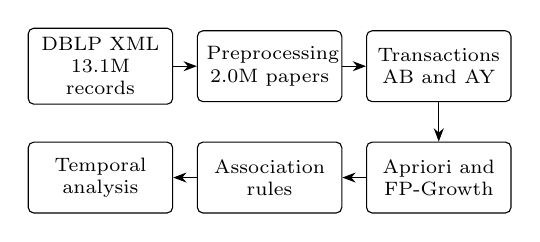
\begin{tikzpicture}[box/.style={draw,rounded corners=2pt,font=\scriptsize,align=center,minimum height=0.9cm,text width=1.6cm},>=Stealth]
\node[box] (a) {DBLP XML\\13.1M records};
\node[box,right=0.3cm of a] (b) {Preprocessing\\2.0M papers};
\node[box,right=0.3cm of b] (c) {Transactions\\AB and AY};
\node[box,below=0.5cm of c] (d) {Apriori and\\FP-Growth};
\node[box,left=0.3cm of d] (e) {Association\\rules};
\node[box,left=0.3cm of e] (f) {Temporal\\analysis};
\draw[->] (a)--(b); \draw[->] (b)--(c); \draw[->] (c)--(d); \draw[->] (d)--(e); \draw[->] (e)--(f);
\end{tikzpicture}
\caption{Overview of the mining pipeline.}
\label{fig:pipeline}
\end{figure}

\subsection{Preprocessing}
We parse the XML in a streaming fashion and keep \texttt{inproceedings} from 2015 to 2025. We then (1) drop records without key, title, year or author (2,255 records), (2) check year validity, (3) remove front matter such as prefaces (1 record), (4) take the venue from the DBLP key, because the \texttt{booktitle} field has many spellings (for example 165 variants for MICCAI), with a few aliases merged (nips to NeurIPS) and \texttt{booktitle} as a fallback when the key has no venue, (5) normalize author names with Unicode NFKC and whitespace cleanup while keeping DBLP disambiguation suffixes, and (6) remove duplicates by key and by content signature of title, year, venue and author set (1,208 records).

\subsection{Transactional Databases}
Let $V$ be the set of venues used as items. In the AB model, one transaction per author contains all venues in which that author published during 2015--2025. In the AY model, one transaction exists per (author, year) pair. Only venues with at least 200 papers become items. Single-item transactions stay in the database so that support is computed over all authors, but they cannot produce rules.

\subsection{Apriori}
Apriori generates candidate $k$-itemsets from frequent $(k-1)$-itemsets and prunes any candidate with an infrequent subset. Our implementation counts support with vertical bitsets, with join and prune steps. It was checked against mlxtend on a 50,000-transaction sample at 1\% support, where itemsets and supports were identical.

\subsection{FP-Growth}
Transactions are inserted into an FP-tree ordered by item frequency. Mining proceeds recursively over conditional pattern bases, so no candidate itemsets are generated. Our own implementation was validated against mlxtend in the same test.

\subsection{Association Rules}
With $D$ the set of transactions and $X$, $Y$ sets of venues,
\begin{align}
\mathrm{supp}(X) &= \frac{|\{T\in D : X\subseteq T\}|}{|D|},\\
\mathrm{conf}(X\Rightarrow Y) &= \frac{\mathrm{supp}(X\cup Y)}{\mathrm{supp}(X)},\\
\mathrm{lift}(X\Rightarrow Y) &= \frac{\mathrm{conf}(X\Rightarrow Y)}{\mathrm{supp}(Y)}.
\end{align}
Rules are generated from every frequent itemset with a minimum confidence of 50\%. We rank rules by lift, because a lift above 1 means $X$ and $Y$ occur together more often than expected if they were independent.

\subsection{Temporal Analysis}
We split the AY database into 2015--2017, 2018--2020, 2021--2023 and 2024--2025, mine each with the same relative minimum support, and compare rules across periods: rules that persist, new rules, lost rules, and lift change on shared rules. To test RQ5, we also computed a group-level lift between three manually defined venue groups (NLP: ACL, EMNLP, NAACL, EACL, COLING, LREC, CoNLL; ML: NeurIPS, ICML, ICLR, AISTATS, UAI, COLT, AAAI, IJCAI; CV: CVPR, ICCV, ECCV, WACV, BMVC, ACCV). It is the probability that a transaction contains a venue of both groups divided by the product of the two single-group probabilities.

\section{Experimental Setup}
Table~\ref{tab:params} lists the parameters needed to reproduce the experiments.

\begin{table}[t]
\caption{Experimental Parameters}
\label{tab:params}
\centering
\footnotesize
\begin{tabular}{p{2.4cm}p{5.0cm}}
\toprule
Parameter & Value \\
\midrule
Environment & Google Colab, Python 3.13, lxml, pandas, NumPy, pyarrow, mlxtend \\
DBLP release & Downloaded 21 Nov 2026 \\
Data period & 2015--2025 \\
Item threshold & 200 papers per venue (1,792 of 4,494 venues; 92.5\% of paper-author rows) \\
Minimum support & 0.1\%, 0.5\%, 1\%, 2\% \\
Minimum confidence & 50\% \\
Metrics & Number of itemsets and rules; execution time as an additional measure \\
Random seed & 42 \\
Temporal periods & 2015--2017, 2018--2020, 2021--2023, 2024--2025 \\
Temporal support & 0.05\% of transactions in each period (AY) \\
\bottomrule
\end{tabular}
\end{table}

\section{Results and Discussion}
\subsection{Preprocessing Results}
The raw data was already clean: preprocessing left 2,000,916 of 2,004,380 papers (99.8\%). Some 2,666 records carry a year that differs from the proceedings year, and we kept the DBLP year field. Papers per year grow from 161,287 in 2015 to 213,645 in 2024. The venue distribution has a long tail: 4,494 venues exist, but the 1,792 venues with at least 200 papers already cover 91.5\% of all papers.

\subsection{Conference Popularity (RQ1)}
NeurIPS ranks first by papers (25,455) and by unique authors (57,800), so the top rank agrees across both measures (Table~\ref{tab:top10}). Eight of the top ten venues appear in both rankings, and the Spearman correlation between the two rankings is 0.987 over all venues and 0.857 over the top 50. The rankings differ for some venues: AAAI is sixth by papers but third by authors, and ICC is tenth by papers but nineteenth by authors. Growth is uneven (Fig.~\ref{fig:trend}): NeurIPS grows 13.2 times from 440 papers in 2015 to 5,823 in 2025 and EMNLP 10.8 times, while all papers grow only 1.24 times. IGARSS and EMBC show zero papers in 2025, most likely because they were not yet indexed in the release we used, so their 2025 counts should be read with care.

\begin{table}[t]
\caption{Top-10 Venues by Papers and by Unique Authors}
\label{tab:top10}
\centering
\footnotesize
\begin{tabular}{rlrlr}
\toprule
Rank & By papers & Papers & By authors & Authors \\
\midrule
1 & NeurIPS & 25,455 & NeurIPS & 57,800 \\
2 & CVPR & 22,752 & CVPR & 47,664 \\
3 & ICASSP & 21,606 & AAAI & 46,435 \\
4 & HCI & 19,912 & ICASSP & 42,060 \\
5 & IGARSS & 19,685 & EMBC & 39,319 \\
6 & AAAI & 19,276 & HCI & 37,884 \\
7 & CHI & 14,834 & IGARSS & 35,229 \\
8 & EMNLP & 14,814 & EMNLP & 33,957 \\
9 & EMBC & 14,677 & ICML & 31,896 \\
10 & ICC & 14,329 & ICLR & 31,315 \\
\bottomrule
\end{tabular}
\end{table}

\begin{figure}[t]
\centering
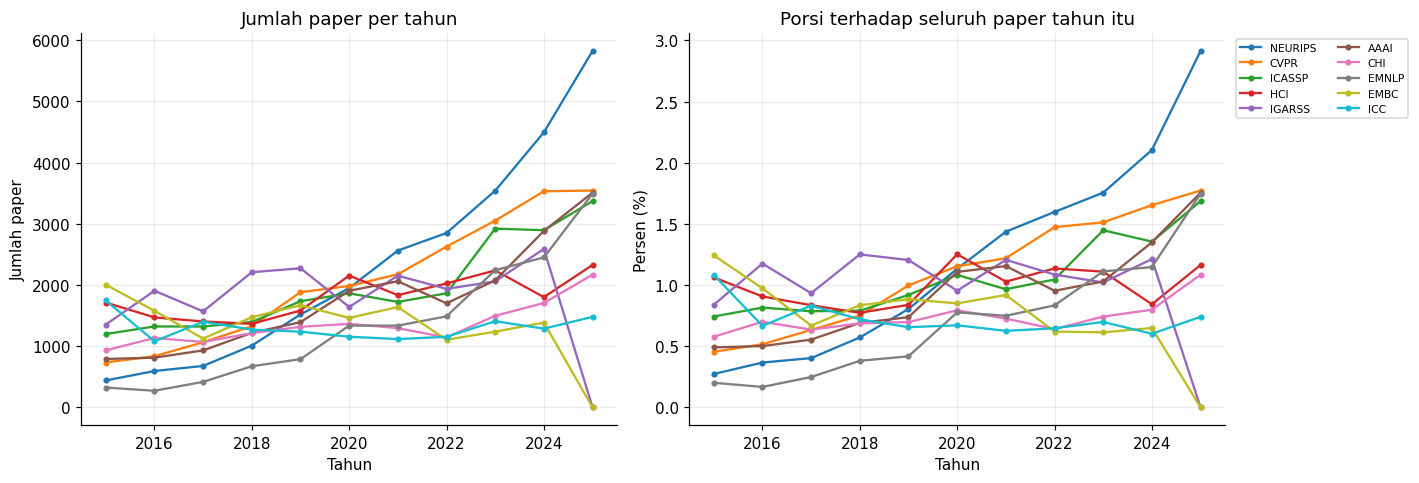
\includegraphics[width=\columnwidth]{fig_trend.png}
\caption{Papers per year (left) and share of all papers in that year (right) for the ten venues with the most papers.}
\label{fig:trend}
\end{figure}

\subsection{Transactional Databases (RQ3)}
The AB database has 1,711,743 transactions with 2.57 venues on average, and the AY database has 3,826,859 transactions with 1.56 venues on average. Single-venue transactions make up 59.0\% of AB and 71.8\% of AY, so 702,200 and 1,080,973 transactions can contribute to rules. AB reflects an author's whole period and therefore holds more co-occurrence (18.1 million venue pairs against 5.1 million in AY, and up to 289 venues in one transaction). AY captures yearly habits but gives productive authors many transactions (2.24 per author on average).

\subsection{Frequent Patterns}
The number of frequent itemsets falls quickly as minimum support rises (Table~\ref{tab:itemsets}). At 2\% only seven single venues remain; pairs appear at 1\% or lower and triples only at 0.5\% or lower (ICLR, ICML and NeurIPS). The most frequent pair is ICML with NeurIPS (1.08\% of authors), followed by ICLR with NeurIPS, AAAI with NeurIPS, CVPR with NeurIPS, CVPR with ICCV, and ACL with EMNLP. These pairs mostly connect venues of the same topic (machine learning, vision, language); ICRA with IROS is a robotics example.

\begin{table}[t]
\caption{Frequent Itemsets by Minimum Support (AB)}
\label{tab:itemsets}
\centering
\footnotesize
\begin{tabular}{lrrrr}
\toprule
Itemset size & 0.1\% & 0.5\% & 1\% & 2\% \\
\midrule
1-itemsets & 623 & 76 & 31 & 7 \\
2-itemsets & 439 & 23 & 2 & 0 \\
3-itemsets & 391 & 1 & 0 & 0 \\
4 or more & 243 & 0 & 0 & 0 \\
Total & 1,696 & 100 & 33 & 7 \\
\bottomrule
\end{tabular}
\end{table}

\subsection{Association Rules (RQ2)}
At 0.1\% support and 50\% confidence, the AB database yields 1,614 rules with lift between 14.9 and 162 (median 33.6). All lifts are far above 1, so these venues rarely co-occur by chance. The strongest rule, ECCV, MM and NeurIPS implying AAAI, CVPR and ICCV (lift 162, confidence 0.61), describes a cluster of authors working across vision and machine learning (Table~\ref{tab:rules}). Among single-venue rules the highest lifts are ECOC $\Rightarrow$ OFC (75.3, optical communications), ASRU $\Rightarrow$ INTERSPEECH (69.7, speech), and EACL $\Rightarrow$ ACL (34.4, language).

High support does not mean high lift (Fig.~\ref{fig:lift}). ICML $\Rightarrow$ NeurIPS has the highest support (1.08\%) but a lift of only 17.2, while ECOC $\Rightarrow$ OFC has a support of 0.26\% and a lift of 75.3. The Spearman correlation between rule support and lift is $-0.195$, and between consequent support and lift it is $-0.913$, so rare consequents tend to give large lift. Support measures how many authors follow a pattern, confidence the chance that an author of $X$ also publishes in $Y$, and lift how much stronger that is than chance.

\begin{table}[t]
\caption{Top Rules by Lift (AB, 0.1\% Support, 50\% Confidence)}
\label{tab:rules}
\centering
\footnotesize
\begin{tabular}{p{3.9cm}rrr}
\toprule
Rule & Supp. & Conf. & Lift \\
\midrule
ECCV, MM, NeurIPS $\Rightarrow$ AAAI, CVPR, ICCV & 0.0011 & 0.613 & 162.0 \\
CVPR, ECCV, ICML $\Rightarrow$ ICCV, ICLR, NeurIPS & 0.0011 & 0.502 & 160.9 \\
CVPR, ICCV, ICML, NeurIPS $\Rightarrow$ ECCV, ICLR & 0.0011 & 0.514 & 149.0 \\
ECOC $\Rightarrow$ OFC & 0.0026 & 0.665 & 75.3 \\
ASRU $\Rightarrow$ INTERSPEECH & 0.0011 & 0.727 & 69.7 \\
\bottomrule
\end{tabular}
\end{table}

\begin{figure}[t]
\centering
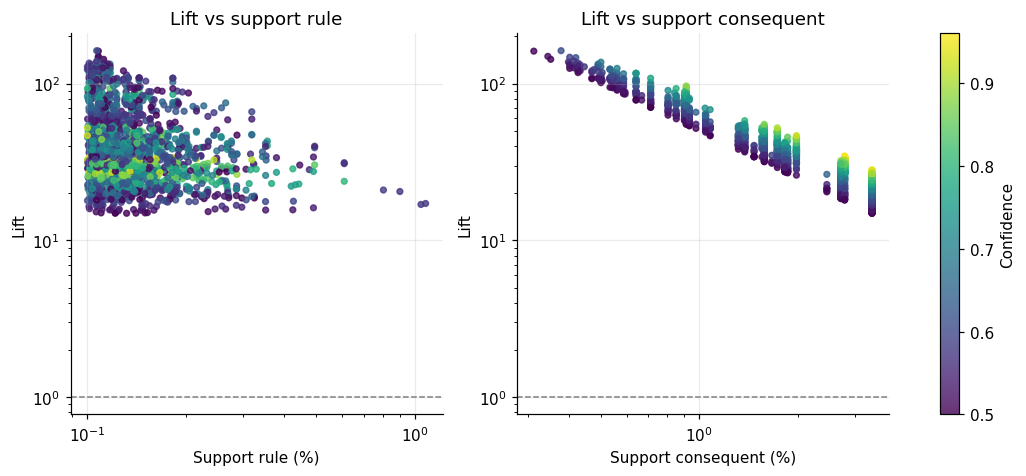
\includegraphics[width=\columnwidth]{fig_lift.png}
\caption{Lift against rule support (left) and against consequent support (right); color shows confidence.}
\label{fig:lift}
\end{figure}

\subsection{Algorithm Comparison (RQ4)}
Apriori and FP-Growth return identical frequent itemsets at every minimum support, and both match mlxtend on a sample (Table~\ref{tab:algo}). Lowering the support increases itemsets and rules sharply: only 7 rules remain at 0.5\% against 1,614 at 0.1\%. Execution time depends on implementation, and our Apriori uses bitset counting. Under that implementation FP-Growth is faster at 0.1\% (11.0 s against 17.7 s), where itemsets are many, while Apriori is faster at higher support (0.06 to 0.56 s against 0.53 to 2.15 s) because FP-Growth pays for building its tree (Fig.~\ref{fig:runtime}). For low support on a large dataset such as DBLP, FP-Growth is the more suitable choice; since the outputs are identical, this is a question of cost only.

\begin{table}[t]
\caption{Apriori versus FP-Growth (AB)}
\label{tab:algo}
\centering
\footnotesize
\begin{tabular}{lrrrr}
\toprule
Min. supp. & Itemsets & Rules & Apriori (s) & FP-Growth (s) \\
\midrule
0.1\% & 1,696 & 1,614 & 17.73 & 10.96 \\
0.5\% & 100 & 7 & 0.56 & 2.15 \\
1\% & 33 & 2 & 0.11 & 0.93 \\
2\% & 7 & 0 & 0.06 & 0.53 \\
\bottomrule
\end{tabular}
\end{table}

\begin{figure}[t]
\centering
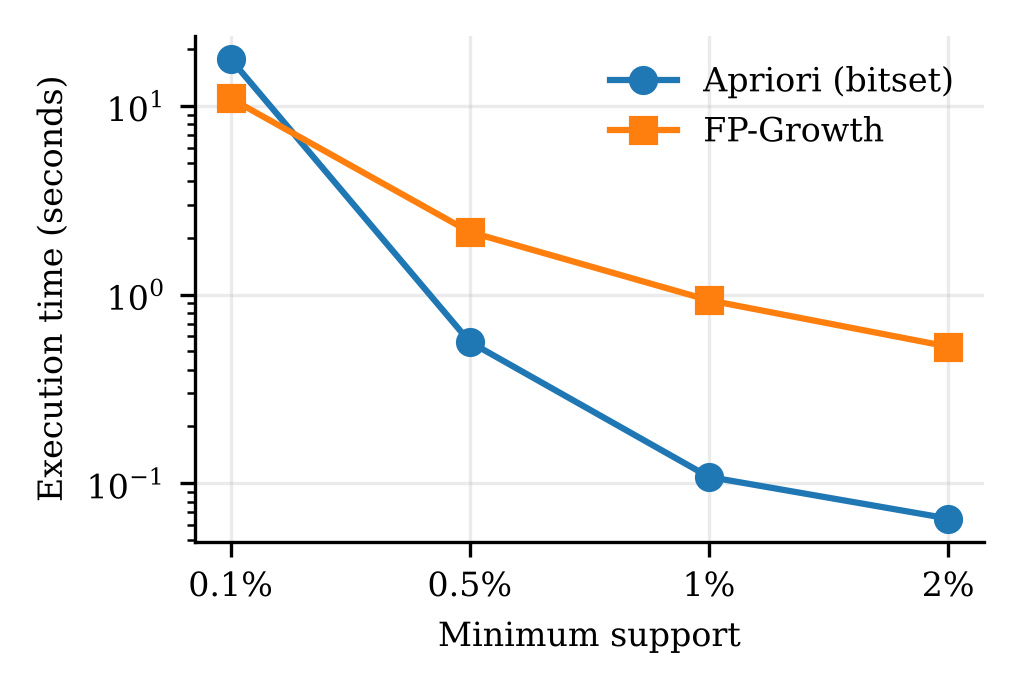
\includegraphics[width=0.85\columnwidth]{fig_runtime.png}
\caption{Execution time of Apriori and FP-Growth against minimum support (log scale).}
\label{fig:runtime}
\end{figure}

\subsection{Temporal Analysis (RQ5)}
Multi-venue patterns increase over time (Table~\ref{tab:temporal}). Pairs grow from 52 to 305, triples from 2 to 227, and itemsets with four or more venues appear only in 2024--2025 (97). Rules grow from 2 to 324. In 2015--2017 the top pairs come from communications and robotics (GLOBECOM with ICC, AMCC with CDC, ICRA with IROS); in 2021--2025 they come from AI (ICML with NeurIPS, ICLR with NeurIPS, ACL with EMNLP, CVPR with NeurIPS). The new rules in 2024--2025 include links between NLP and ML venues, for example AAAI, EMNLP and ICLR implying ACL and NeurIPS (lift 86.1).

The hypothesis that NLP--ML association strengthens is only partly supported. The group-level lift between NLP and ML falls from 5.35 to 2.63, and between CV and ML from 5.05 to 2.89, while NLP and CV rises slightly from 1.41 to 1.77 (Fig.~\ref{fig:grouplift}). A likely reason is that the ML group grew very quickly, so more joint publication is less surprising relative to chance. The two readings are not in conflict: co-publication increased in absolute terms, but the association relative to independence decreased.

\begin{table}[t]
\caption{Itemsets and Rules per Period (AY, 0.05\% Support)}
\label{tab:temporal}
\centering
\footnotesize
\begin{tabular}{lrrrr}
\toprule
Measure & 15--17 & 18--20 & 21--23 & 24--25 \\
\midrule
Transactions (thousands) & 855 & 1,014 & 1,121 & 837 \\
Frequent itemsets & 910 & 868 & 926 & 1,267 \\
2-itemsets & 52 & 91 & 148 & 305 \\
3-itemsets & 2 & 6 & 31 & 227 \\
4 or more & 0 & 0 & 0 & 97 \\
Rules & 2 & 5 & 26 & 324 \\
\bottomrule
\end{tabular}
\end{table}

\begin{figure}[t]
\centering
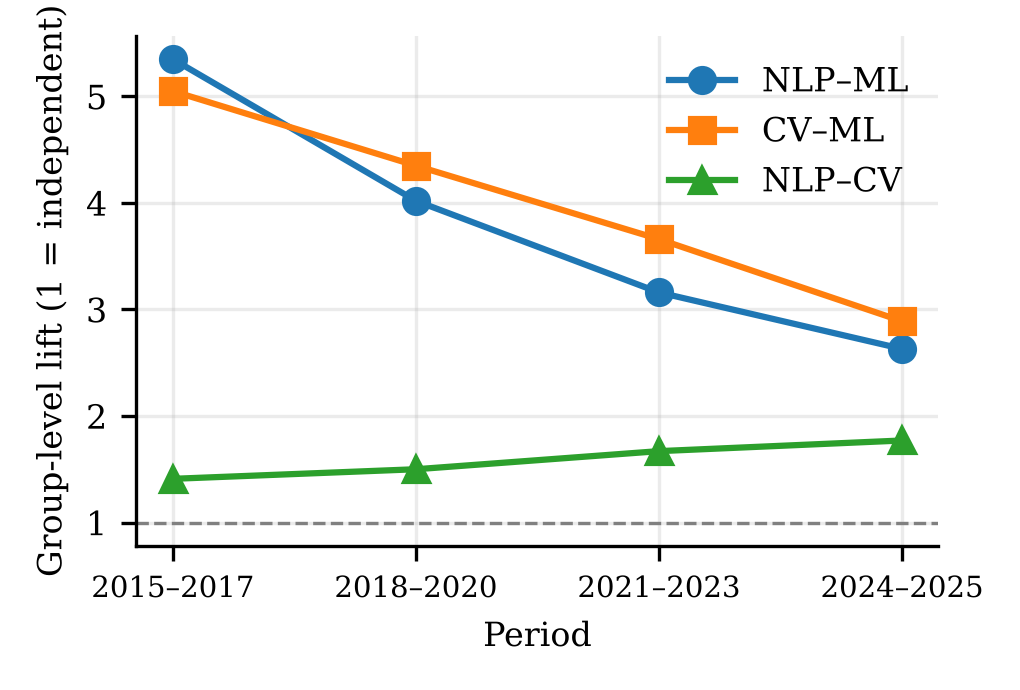
\includegraphics[width=0.85\columnwidth]{fig_group_lift.png}
\caption{Group-level lift between venue groups in each period.}
\label{fig:grouplift}
\end{figure}

Two cautions apply. First, at this threshold the early periods have very few rules (2 and 5), so no rule appears in all four periods and rule overlap between periods is weak (Jaccard 0.11 or less); the counts of itemsets and the group-level lift are more robust than rule overlap. A lower temporal support should be tried before drawing conclusions about individual rules. Second, the last period covers only two years, and some venues of 2025 are not yet indexed. These are associations and do not show that LLMs caused the change.

\subsection{Author-Based versus Author-Year-Based (RQ3)}
At the same minimum support, AB yields 1,696 itemsets and 1,614 rules, while AY yields 380 itemsets and only 3 rules (Table~\ref{tab:abay}). The top venue pairs are similar (18 of the 20 highest-support pairs coincide), but rule overlap is small (Jaccard 0.002; three shared rules with the same lift order). Thus the strongest pairs are consistent across models, but AB captures long-run, multi-venue patterns with very high lift, while AY reflects yearly habits and is more conservative (top lift 25.4).

\begin{table}[t]
\caption{Author-Based versus Author-Year-Based (Same Minimum Support)}
\label{tab:abay}
\centering
\footnotesize
\begin{tabular}{lrr}
\toprule
Measure & AB & AY \\
\midrule
Transactions & 1,711,743 & 3,826,859 \\
Frequent itemsets & 1,696 & 380 \\
Itemsets with 2+ venues & 1,073 & 53 \\
Rules & 1,614 & 3 \\
Top rule lift & 162.0 & 25.4 \\
\bottomrule
\end{tabular}
\end{table}

\section{Limitations and Threats to Validity}
\begin{itemize}
\item Popularity is publication activity, not quality or citations.
\item Author disambiguation relies on DBLP; merged or split identities remain possible, and person-record aliases are not used.
\item Some 2025 venues (IGARSS, EMBC) show zero papers, probably because they are not yet indexed, which biases 2025 counts and the last period.
\item Only venues with at least 200 papers are items (1,792 of 4,494, covering 92.5\% of paper-author rows), and single-venue transactions cannot produce rules.
\item AB merges the whole period, hiding yearly patterns; AY gives productive authors many transactions.
\item At the temporal support of 0.05\%, early periods have only 2 and 5 rules, so rule-level comparison across periods is weak.
\item The venue groups (NLP, ML, CV) are defined by hand, and the 2024--2025 period has only two years.
\item Associations are not causal; the shift between periods does not prove that LLMs caused it.
\item Colab memory limits low minimum support, and timing results depend on our implementations.
\end{itemize}

\section{Conclusion}
NeurIPS is the most popular venue by both papers (25,455) and unique authors (57,800). It also forms the most frequent pair, ICML with NeurIPS (1.08\% of authors), but the strongest associations by lift appear between smaller, specialized venues such as ECOC and OFC (75.3) and between sets of vision and ML venues (up to 162), so popularity does not imply the strongest association. The AB model finds far more patterns than the AY model (1,614 against 3 rules at the same support), although both agree on the leading pairs. Apriori and FP-Growth give identical results, with FP-Growth faster at low support, which makes it the better choice for DBLP. Over time, multi-venue patterns grow from 2 to 324 rules and the center of association shifts from communications and robotics to AI, but the hypothesis of stronger NLP--ML association is only partly supported, since group-level lift falls while rules linking NLP and ML venues appear. Future work includes citation-weighted associations, journals, analysis by subfield, lower temporal support with complete 2025 data, and sequential temporal rules.

\section*{Acknowledgment}
The authors thank the DBLP team at Schloss Dagstuhl and the University of Trier for providing the data.

\begin{thebibliography}{00}
\bibitem{dblp} ``DBLP computer science bibliography,'' Schloss Dagstuhl and University of Trier. [Online]. Available: https://dblp.org/. Accessed: Nov. 21, 2026.
\bibitem{apriori} R. Agrawal and R. Srikant, ``Fast algorithms for mining association rules,'' in \textit{Proc. 20th Int. Conf. Very Large Data Bases (VLDB)}, 1994, pp. 487--499.
\bibitem{fpgrowth} J. Han, J. Pei, and Y. Yin, ``Mining frequent patterns without candidate generation,'' in \textit{Proc. ACM SIGMOD Int. Conf. Management of Data}, 2000, pp. 1--12.
\bibitem{kim} J. Kim, ``Author-based analysis of conference versus journal publication in computer science,'' arXiv:1806.10674, 2018.
\bibitem{biryukov} M. Biryukov and C. Dong, ``Analysis of computer science communities based on DBLP,'' arXiv:1012.5396, 2010.
\bibitem{kull} L. K\"ull, ``Analyzing the state of computer science research with the DBLP Discovery Dataset,'' arXiv:2212.00629, 2022.
\bibitem{schommer} C. Schommer, ``A simple framework to typify social bibliographic communities,'' arXiv:0809.2818, 2008.
\end{thebibliography}

\end{document}
